%%%%%%%%%%%%%%%%%%%%%%%%%%%%%%%%%%%%%%%%%%%%%%%%%%%%%%%%%%%%%%%%%%%%%%%%%%%%%%%%
%2345678901234567890123456789012345678901234567890123456789012345678901234567890
%        1         2         3         4         5         6         7         8

% \documentclass[letterpaper, 10 pt, conference]{ieeeconf}  % Comment this line 
% out if you need a4paper

\documentclass[usletter, 10pt, conference]{ieeeconf}      % Use this line for a4 
% paper
% \usepackage[backend=bibtex,bibstyle=ieee,citestyle=numeric-comp]{biblatex}
% \bibliography{icra17radulescu}
\usepackage{graphicx}\graphicspath{{figures/}}
\usepackage{todonotes}
\renewcommand{\todo}[1]{\textcolor{magenta}{[TODO: #1]}}
\usepackage{amsmath,amsfonts,euscript,amscd,amssymb}
% \numberwithin{equation}{chapter}
% \usepackage{caption}
% \captionsetup[figure]{figurewithin=chapter}
% \numberwithin{table}{chapter}
% \usepackage{multirow, setspace} 
% \usepackage{subfigure}
\usepackage{graphicx}
\usepackage{caption}
\usepackage{subcaption}
\usepackage{algorithm}
\usepackage{algorithmic} 
\usepackage{epsfig}
\usepackage{enumerate}
\usepackage{gensymb}
\usepackage{notoccite}
\usepackage{svg}
\usepackage{url}
\pdfminorversion=4
% \usepackage[noadjust]{cite}
% \usepackage{cite}
% \usepackage[utf8x]{inputenc}
% % functions
% \newcommand{\estimated}[1]{\hat{#1}}
% \newcommand{\qindent}{\hspace{4em}}
% 
% % general


\newcommand{\R}{\mathbb{R}}
% rigid body dynamics
\newcommand{\qdot}{\dot{q}}             % joint velocity
\newcommand{\qddot}{\ddot{q}}           % joint acceleration
\newcommand{\bq}{\mathbf{q}}            % (bold) joint position
\newcommand{\bqdot}{\dot{\bq}}          % (bold) joint velocity
\newcommand{\bqddot}{\ddot{\bq}}        % (bold) joint acceleration
\newcommand{\bM}{\mathbf{M}}            % inertia matrix
\newcommand{\bMt}{\tilde{\mathbf{M}}} 
\newcommand{\bh}{\mathbf{h}}    
\newcommand{\bS}{\mathbf{S}}    
\newcommand{\VF}{\mathbf{V}}  
\newcommand{\bR}{\mathbf{R}}  
\newcommand{\bQ}{\mathbf{Q}}  
\newcommand{\bJ}{\mathbf{J}} 
\newcommand{\bzero}{\mathbf{0}} 
\newcommand{\bP}{\mathbf{P}}  
\newcommand{\traj}{\mathbf{\tau}}
\newcommand{\bPsi}{\mathbf{\Psi}} 

\newcommand{\Cn}{\mathcal{C}}

 \newcommand{\bC}{\mathbf{C}} 
\newcommand{\bg}{\mathbf{g}} 
\newcommand{\bG}{\mathbf{G}} 
\newcommand{\bw}{\mathbf{w}} 
\newcommand{\Bfc}{\mathbf{f_c}} 
\newcommand{\bz}{\mathbf{z}}

\newcommand{\bV}{\mathbf{V}}    
\newcommand{\bD}{\mathbf{D}}     

\newcommand{\bI}{\mathbf{I}}   
\newcommand{\bv}{\mathbf{v}}            % velocities at contact
\newcommand{\blambda}{\mathbf{Y}} % forces at contact
\newcommand{\bK}{\mathbf{K}}            % Jacobian of mapping from generalised to contact 
\newcommand{\bKt}{\tilde{\mathbf{K}}}            % Jacobian of mapping from generalised to contact 
\newcommand{\bc}{\mathbf{c}}   		% compacting term (known terms)
\newcommand{\bff}{\mathbf{f}}   		% compacting term (contact impulse)
\newcommand{\bct}{\tilde{\mathbf{c}}}   		% compacting term (known terms)
\newcommand{\bA}{\mathbf{A}}     
\newcommand{\ba}{\mathbf{a}}     
\newcommand{\bF}{\mathbf{F}}     
\newcommand{\bB}{\mathbf{B}}    

\newcommand{\bl}{\mathbf{l}}  
\newcommand{\bL}{\mathbf{L}}  
\newcommand{\bLbar}{\bar {\mathbf{L}} }

\newcommand{\btau}{\boldsymbol{\tau}}   % (bold) torque

%optimal control
\newcommand{\dimU}{m} %dimensionality of control
\newcommand{\f}{\mathcal{F}} %dynamics function
\newcommand{\F}{\mathbf{F}} %dynamics function
\newcommand{\bu}{\mathbf{u}}  %control vector
\newcommand{\bx}{\mathbf{x}}  %state
\newcommand{\bp}{\mathbf{p}}  %state
\newcommand{\bs}{\mathbf{s}}  %state
% \newcommand{\bS}{\mathbf{S}}  %state
\newcommand{\tc}{\rho} %terminal cost
\newcommand{\rc}{r} %running cost
\newcommand{\J}{\mathbf{J}} %cost function
\newcommand{\dimX}{n}
\newcommand{\bxdot}{\dot{\bx}}          % state time derivative
\newcommand{\g}{\mathcal{G}} %stochasticity in dynamics

\newcommand{ \probability}{\mathsf{p}}            % 
\newcommand{\lambdaLM}{\beta}            % LM scalar iLQG

\newcommand{\tp}{\mathit{tp}}
\newcommand{\z}{\mathit{z}}
\newcommand{\bxp}{\bx'}  
\newcommand{\scost}{\mathit{o}} % state cost function

\newcommand{\mbf}{\mathbf}

\newcommand{\gMAT}{\mathbf{G}}

\newcommand{\bbx}   {\bar{\bx}}         % nominal state sequence
\newcommand{\bbu}   {\bar{\bu}}         % nominal command sequence

\newcommand{\fx}   {\f_\bx}             % dynamics function derivative w.r.t. x
\newcommand{\fu}   {\f_\bu}             % dynamics function derivative w.r.t. u
\newcommand{\hx}   {\tc_\bx}              % terminal cost function derivative w.r.t. x
\newcommand{\hxx}  {\tc_{\bx\bx}}         % terminal cost function 2nd derivative w.r.t. x
\newcommand{\lx}   {\rc_\bx}              % running cost function derivative w.r.t. x
\newcommand{\lu}   {\rc_\bu}              % running cost function derivative w.r.t. u
\newcommand{\lxx}  {\rc_{\bx\bx}}         % running cost function 2nd derivative w.r.t. x
\newcommand{\luu}  {\rc_{\bu\bu}}         % running cost function 2nd derivative w.r.t. u
\newcommand{\lxu}  {\rc_{\bx\bu}}         % running cost function cross derivative

\newcommand{\xbar}{\bar{\mathbf{x}}}
\newcommand{\ubar}{\bar{\mathbf{u}}}
\newcommand{\Jbar}{\bar{\J}}

\newcommand{\Jxx}  {\J_{\bx\bx}}         % running cost function 2nd derivative w.r.t. x
\newcommand{\Juu}  {\J_{\bu\bu}}         % running cost function 2nd derivative w.r.t. u
\newcommand{\Jxu}  {\J_{\bx\bu}} 

\newcommand{\utilde}{\tilde{\mathbf{u}}}
\newcommand{\xtilde}{\tilde{\mathbf{x}}}
\newcommand{\Jtilde}{\tilde{\J}}
\newcommand{\Hfix}{\mathcal{H}}
\newcommand{\Ham}{\mathbf{H}}


\newcommand{\dt}{\mathrm{d}t}


\def \BDelta { {\bf \Delta} }
\def \Real { \mathbb{R} }

 \newcommand{\dimQ}{\dimX}
\newcommand{\dimC}{\dimU}
%%%%%%%%%%% useful math stuff %%%%%%%%%%%
\newcommand{\twovec}[2]{\left[\begin{array}{c}
                                  #1\\ #2\\
                            \end{array}
                       \right]}
\newcommand{\threevec}[3]{\left[\begin{array}{c}
                                  #1\\ #2\\ #3 \\
                            \end{array}
                       \right]}
\newcommand{\fourvec}[4]{\left[\begin{array}{c}
                                  #1\\ #2\\ #3 \\ #4\\
                            \end{array}
                       \right]}

\newcommand{\tworvec}[2]{\left[\begin{array}{cc}
                                  #1 & #2\\
                            \end{array}
                       \right]}

\newcommand{\threervec}[3]{\left[\begin{array}{ccc}
                                  #1 & #2 & #3\\
                            \end{array}
                       \right]}

\newcommand{\fourrvec}[4]{\left[\begin{array}{cccc}
                                  #1 & #2 & #3 & #4\\
                            \end{array}
                       \right]}

\newcommand{\twovect}[2]{[\;#1,\;#2\;]^T}
\newcommand{\threevect}[3]{[\;#1,\;#2,\;#3\;]^T}
\newcommand{\fourvect}[4]{[\;#1,\;#2,\;#3,\;#4\;]^T}
\newcommand{\twomatrix}[4]{ \left[\begin{array}{cc}
                                   #1 & #2\\
                                   #3 & #4\\
                                 \end{array}
                           \right]}
\newcommand{\threematrix}[9]{ \left[\begin{array}{ccc}
                                   #1 & #2 & #3 \\
                                   #4 & #5 & #6 \\
				   #7 & #8 & #9 \\
                                 \end{array}
                           \right]}
\newcommand{\eqdef}{\stackrel{\rm def}{=}}
\newcommand{\diag}{\mathrm{diag}}

% partial derivatives
\newcommand{\partiald}[2]{
\frac{\partial #1}{\partial #2}}

\newcommand{\partialtwod}[2]{
\frac{\partial^{2} #1}{\partial #2}}

%%% definition of boldmath letters %%%

   %%% lower case Greek letters
\def \Balpha      { {\mbox{\boldmath $\alpha$}}}
\def \Bbeta       { {\mbox{\boldmath $\beta$}}}
\def \Bgamma      { {\mbox{\boldmath $\gamma$}}}
\def \Bdelta      { {\mbox{\boldmath $\delta$}}}
\def \Bepsilon    { {\mbox{\boldmath $\epsilon$}}}
\def \Bvarepsilon { {\mbox{\boldmath $\varepsilon$}}}

\def \Bzeta       { {\mbox{\boldmath $\zeta$}}}
\def \Beta        { {\mbox{\boldmath $\eta$}}}
\def \Btheta      { {\mbox{\boldmath $\theta$}}}
\def \Bvartheta   { {\mbox{\boldmath $\vartheta$}}}
\def \Biota       { {\mbox{\boldmath $\iota$}}}

\def \Bkappa      { {\mbox{\boldmath $\kappa$}}}
\def \Blambda     { {\mbox{\boldmath $\lambda$}}}
\def \Bmu         { {\mbox{\boldmath $\mu$}}}
\def \Bnu         { {\mbox{\boldmath $\nu$}}}
\def \Bxi         { {\mbox{\boldmath $\xi$}}}
\def \Bomicron    { {\mbox{\boldmath $o$}}}

\def \Bpi         { {\mbox{\boldmath $\pi$}}}
\def \Bphi        { {\mbox{\boldmath $\phi$}}}
\def \Brho        { {\mbox{\boldmath $\rho$}}}
\def \Bvarrho     { {\mbox{\boldmath $\varrho$}}}
\def \Bsigma      { {\mbox{\boldmath $\sigma$}}}
\def \Bvarsigma   { {\mbox{\boldmath $\varsigma$}}}

\def \Btau        { {\mbox{\boldmath $\tau$}}}
\def \Bupsilon    { {\mbox{\boldmath $\upsilon$}}}
\def \Bphi        { {\mbox{\boldmath $\phi$}}}
\def \Bvarphi     { {\mbox{\boldmath $\varphi$}}}
\def \Bchi        { {\mbox{\boldmath $\chi$}}}
\def \Bpsi        { {\mbox{\boldmath $\psi$}}}
\def \Bomega      { {\mbox{\boldmath $\omega$}}}


   %%% upper case Greek letters
\def \BAlpha      { {\bf A} }
\def \BBeta       { {\bf B} }
\def \BGamma      { {\bf \Gamma} }
\def \BDelta      { {\bf \Delta} }
\def \BEpsilon    { {\bf E} }

\def \BZeta       { {\bf Z} }
\def \BEta        { {\bf H} }
\def \BTheta      { {\bf \Theta} }
\def \BIota       { {\bf I} }

\def \BKappa      { {\bf K} }
\def \BLambda     { {\bf \Lambda} }
\def \BMu         { {\bf M} }
\def \BNu         { {\bf N} }
\def \BXi         { {\bf \Xi} }
\def \BOmicron    { {\bf O} }

\def \BPi         { {\bf \Pi} }
\def \BPhi        { {\bf \Phi} }
\def \BRho        { {\bf P} }
\def \BSigma      { {\bf \Sigma} }

\def \BTau        { {\bf T} }
\def \BUpsilon    { {\bf \Upsilon} }
\def \BPhi        { {\bf \Phi} }
\def \BChi        { {\bf X} }
\def \BPsi        { {\bf \Psi} }
\def \BOmega      { {\bf \Omega} }

   %%% lower case bold letters
\def \Ba { {\bf a} }
\def \Bb { {\bf b} }
\def \Bc { {\bf c} }
\def \Bd { {\bf d} }
\def \Be { {\bf e} }
\def \Bf { {\bf f} }
\def \Bg { {\bf g} }
\def \Bh { {\bf h} }
\def \Bi { {\bf i} }
\def \Bj { {\bf j} }
\def \Bk { {\bf k} }
\def \Bl { {\bf l} }
\def \Bm { {\bf m} }
\def \Bn { {\bf n} }
\def \Bo { {\bf o} }
\def \Bp { {\bf p} }
\def \Bq { {\bf q} }
\def \Br { {\bf r} }
\def \Bs { {\bf s} }
\def \Bt { {\bf t} }
\def \Bu { {\bf u} }
\def \Bv { {\bf v} }
\def \Bw { {\bf w} }
\def \Bx { {\bf x} }
\def \By { {\bf y} }
\def \Bz { {\bf z} }

   %%% upper case bold letters
\def \BA { {\bf A} }
\def \BB { {\bf B} }
\def \BC { {\bf C} }
\def \BD { {\bf D} }
\def \BE { {\bf E} }
\def \BF { {\bf F} }
\def \BG { {\bf G} }
\def \BH { {\bf H} }
\def \BI { {\bf I} }
\def \BJ { {\bf J} }
\def \BK { {\bf K} }
\def \BL { {\bf L} }
\def \BM { {\bf M} }
\def \BN { {\bf N} }
\def \BO { {\bf O} }
\def \BP { {\bf P} }
\def \BQ { {\bf Q} }
\def \BR { {\bf R} }
\def \BS { {\bf S} }
\def \BT { {\bf T} }
\def \BU { {\bf U} }
\def \BV { {\bf V} }
\def \BW { {\bf W} }
\def \BX { {\bf X} }
\def \BY { {\bf Y} }
\def \BZ { {\bf Z} }

%%%  bold numbers
\def \Bzero { {\bf 0} }
\def \Bone  { {\bf 1} }

%%% Re %%% need \usepackage{amsfonts}
\usepackage{amsfonts}
\def \Real { \mathbb{R} }

\newtheorem{theorem}{Theorem}
\newtheorem{lemma}{Lemma}
\newtheorem{definition}{Definition}

%%% end of math stuff


\IEEEoverridecommandlockouts                              % This command is only 
% needed if 
                                                          % you want to use the 
% \thanks %command

\overrideIEEEmargins                                      % Needed to meet 
% printer requirements.

% See the \addtolength command later in the file to balance the column lengths
% on the last page of the document

% The following packages can be found on http:\\www.ctan.org
%\usepackage{graphics} % for pdf, bitmapped graphics files
%\usepackage{epsfig} % for postscript graphics files
%\usepackage{mathptmx} % assumes new font selection scheme installed
%\usepackage{times} % assumes new font selection scheme installed
%\usepackage{amsmath} % assumes amsmath package installed
%\usepackage{amssymb}  % assumes amsmath package installed

% \title{\LARGE \bf Whole-body Trajectory Optimization for \\ Non-periodic Dynamic 
% Motions on Quadrupedal Systems}

\title{\LARGE \bf Whole-body Trajectory Optimization for Non-periodic Dynamic Motions in Legged Systems}
\author{Andreea Radulescu$^{1}$  Ioannis Havoutis$^{2,3}$ Darwin G. Caldwell$^1$ Claudio Semini$^{1}$ 
% \thanks{*This research is funded by the Fondazione Istituto Italiano di Tecnologia}% <-this % stops a space
\thanks{$^{1}$Department of Advanced Robotics, Istituto Italiano di
Tecnologia, Genova, Italy. \textit{email}: {\tt\small \{andreea.radulescu, darwin.caldwell,  claudio.semini\}@iit.it}}%
\thanks{$^{2}$Robot Learning and Interaction Group, Idiap Research Institute, 
Martigny, Switzerland \textit{email}: {\tt\small ioannis.havoutis@idiap.ch}}%
\thanks{$^{3}$Oxford Robotics Institute, Department of Engineering Science, University of Oxford, United Kingdom. {\tt\small ihavoutis@robots.ox.ac.uk}}%
}


\begin{document}

\maketitle
\thispagestyle{empty}
\pagestyle{empty}

%%%%%%%%%%%%%%%%%%%%%%%%%%%%%%%%%%%%%%%%%%%%%%%%%%%%%%%%%%%%%%%%%%%%%%%%%%%%%%%%
\begin{abstract}
We present a whole-body optimization methodology for non-periodic tasks on quadrupedal systems (rearing and pose recovery). 
This approach delivers solutions involving multiple contacts without 
the need for predefined feet placements. The results obtained show the potential of such methods for 
motion synthesis in the context of complex tasks. The work described has been presented in
detail in \cite{icra17radulescu}.
\end{abstract}

% \begin{keywords}
% \textit{optimization, parametrized policy, multi-legged systems, switching contacts,
% non-periodic movements, quadruped, posture recovery, whole-body trajectory}
% \end{keywords}

\section{Introduction}

A fully autonomous locomotion system would have to complete a heterogeneous range of tasks, some
of which would require non-periodic solutions which could be described as single-shot movements.
Examples in quadrupedal locomotion include rearing, overcoming an obstacle or gap, 
squat-jumping in place, posture and fall recovery. 

Currently, the majority of robotic systems operating in an unsafe, disorganized and cluttered 
environment (e.g., search and rescue missions, disaster response, nuclear decommissioning) have to rely 
heavily on teleoperation in order to achieve their objectives. 
Optimization and learning methodologies could deliver solutions for such scenarios 
by using high-level task specifications, in the form of an evaluation criterion 
of the overall performance of the emerging behavior. 

\section{State of the art}

The relationship between learning and optimization has been under analysis for a long time
\cite{bennett2006interplay,kober2013reinforcement}. However, it is only in the recent past
that their use has been extended to high dimensional problems, common to modern
multi-degree-of-freedom (DoF) robotics applications. 
Various optimization techniques were proposed for dealing with multiple contact events. 
One popular approach is based on online Model Predictive Control (MPC)
\cite{Erez2011,posa_tedrake.IJRR2014}.
Methods such as Policy Improvement with Path Integrals ($PI^2$) \cite{theodorou2010generalized}, 
based on stochastic optimal control principles, were also successful in generating 
optimal solutions for robotic systems \cite{kalakrishnan2011learning, fankhauser2013reinforcement}.
The Covariance Matrix Adaptation (CMA) algorithm \cite{hansen2001completely} 
has been similarly used to generate whole body movements \cite{gehring2016practice}. 

Another major challenge is solving such high-level tasks without the use of 
pre-defined heuristics such as hard-coded sequences or feet 
placements \cite{Winkler2015}. In spite of the significant efforts in the area of fall avoidance, 
comparatively little research has focused
on developing generalized self-righting techniques \cite{ben2008design, kessens2014metric}. 

\section{Our methodology}

We address this issue by providing a generalized approach for 
delivering whole body movement solutions.  
We use a CMA evolution strategy based procedure to address dynamic 
non-periodic tasks for a quadrupedal robotic system: rearing and posture 
recovery. A direct optimization technique on the time-parametrized joint 
or torque trajectories would involve an inconveniently large search 
space. Hence, we use a parametrized policy to encode these profiles, represented as 
a weighted average of Gaussian kernels: $ f(t) = \sum_{i=1}^{M} w_i \phi_i(t)/ \sum_{i=1}^{M} \phi_i(t)$,
% \begin{equation}\small
%  \label{weighted_sum}
%  f(t) = \sum_{i=1}^{M} w_i \phi_i(t)/ \sum_{i=1}^{M} \phi_i(t),
%  \end{equation}
\noindent where $w_i$ are the weights associated with each kernel $\phi_i, \; i \in [1, M]$, defined by:
$\phi_i(t) = exp(- \frac{1}{2 \sigma^2} (t-\mu_i))$.

The CMA algorithm is then used to optimize the weights of all 
policies according to a task specific cost function, applied to the 
whole body trajectory generated through the parametrized policy.
In our experiments we use 12 such representations, one for each DoF of the quadrupedal system. 

% \begin{figure}[t!]
%  \centering
%  \hspace*{-1mm}
%  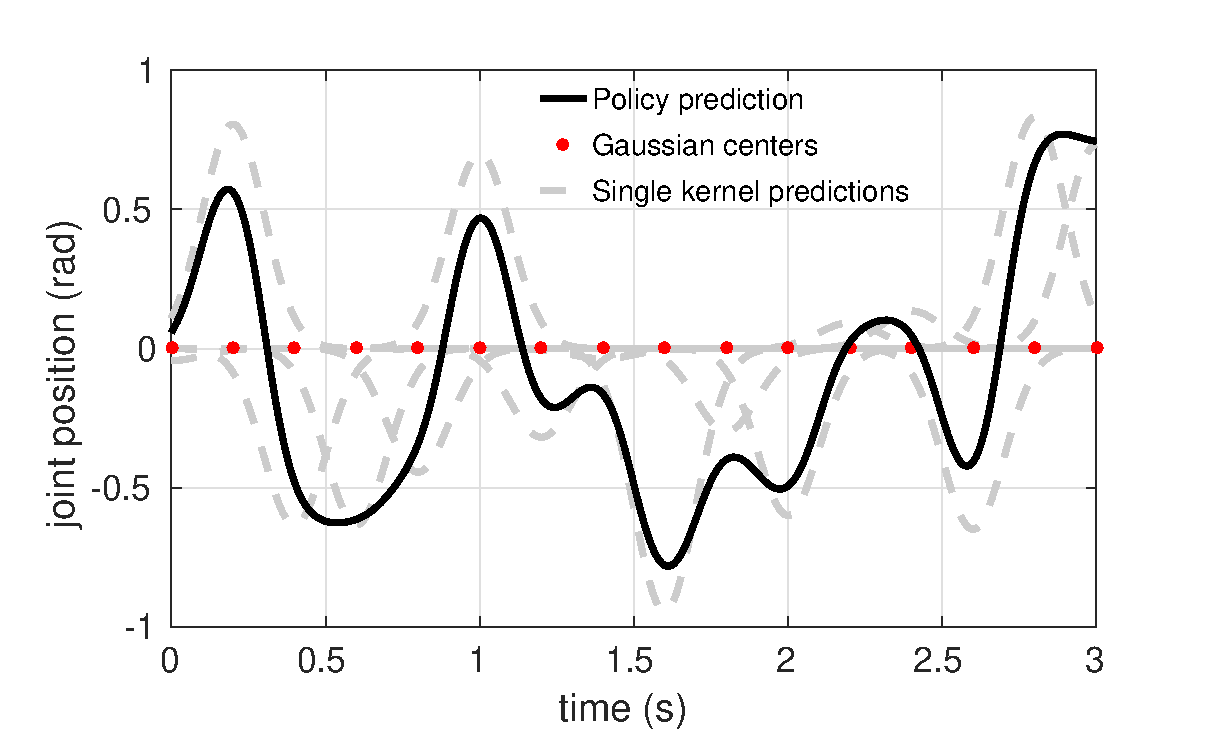
\includegraphics[scale=.4]{example_gr3.eps} 
%  \caption{Example of a policy encoded as a weighted average of 
%  Gaussian kernels: the means $\mu_i$ are equally spaced and the 
%  variances are all fixed to $0.01$ and the weights have been 
%  sampled from $[-1,1]$.}
%   \label{fig:policy_example}
% \end{figure}


\section{Simulation Results}

Using a realistic simulation of the hydraulically actuated HyQ2Max quadruped \cite{semini16tmech}, 
we investigate two distinctive tasks: rearing and posture recovery. We employ a
generalized form for the cost function, while adjusting the relative gains of each term 
according to the current task. Although tuning the relative weights of such cost functions is a manual 
process, a heuristic encoding of the same behavior would require a significantly higher effort.

By exploiting the whole body model in order to obtain the solution, the optimization does not have
to depend upon a pre-specified solution guess and can overcome errors caused by the use of simplified models.
The resultant trajectories and the accuracy with which the user defined goals are achieved are 
reflecting the relative ratios of the weights on the individual cost function terms. 


\section{Conclusion and Future directions}

The approach is able to provide 
trajectory solutions which involve multiple contacts, without any predefined
feet placement heuristics (e.g., contact points, timing or order of succession). 
We aim to extend the methodology to deliver an optimal duration for the given task,
while the final pose is fully determined, based on
subsequent requirements. In the long term we aspire to develop a general tool for generating optimal dynamic 
whole-body motions that are not necessarily periodic in nature.

% \renewcommand{\baselinestretch}{0.9}

\bibliographystyle{IEEEtran}
% \bibliographystyle{ieeetr}
\bibliography{icra17radulescu}

\end{document}
